% !TEX program = XeLaTeX
% !TEX encoding = UTF-8
\documentclass[UTF8,nofonts]{article}
%{ctexart}


%\setCJKmainfont[BoldFont=FandolSong-Bold.otf,ItalicFont=FandolKai-Regular.otf]{FandolSong-Regular.otf}
%\setCJKsansfont[BoldFont=FandolHei-Bold.otf]{FandolHei-Regular.otf}
%\setCJKmonofont{FandolFang-Regular.otf}

\usepackage[ngerman]{babel}
\usepackage[utf8]{inputenc}
\usepackage{url}
\usepackage{cancel}
\usepackage{xspace}
\usepackage{graphicx}
\usepackage{multicol}
\usepackage{multirow}
\usepackage{subfig}
\usepackage{amsmath}
\usepackage{amssymb}
\usepackage[a4paper, width=186mm, top=18mm, bottom=18mm, includeheadfoot]{geometry}
%\usepackage[a4paper, width=140mm, top=18mm, bottom=22mm, includeheadfoot]{geometry}
\usepackage{booktabs}
\usepackage{array}
\usepackage{verbatim}
\usepackage{caption}
\usepackage{natbib}
\usepackage{booktabs}
\usepackage{float}
\usepackage{pdflscape}
\usepackage{mathtools}
\usepackage[usenames, dvipsnames]{xcolor}
\usepackage{afterpage}
\usepackage{pgf}
\usepackage{tikz}
\usepackage{dirtree}
\usepackage[style=american]{csquotes}
\usepackage{amsfonts}
\usepackage{tikz}
\usepackage{tkz-graph}
\usetikzlibrary{arrows,decorations.pathmorphing,automata,positioning,backgrounds,fit,shapes.symbols,chains,intersections}

\newtheorem{definition}{Definition}[section]
\newtheorem{theorem}{Theorem}[section]
\newtheorem{lemma}{Lemma}
\newtheorem{proof}{Proof} [section]



\usepackage[toc, page, title, titletoc, header]{appendix}
\usepackage{marginnote}
\usepackage{tablefootnote}

\addto{\captionsngerman}{\renewcommand{\abstractname}{Kurzdarstellung}}
\renewcommand\appendixname{Anhänge}
\renewcommand\appendixpagename{Anhänge}
\renewcommand\appendixtocname{Anhänge}


\usepackage{perpage} %the perpage package
\MakePerPage{footnote} %the perpage package command

\usetikzlibrary{shapes.geometric}%
\usepackage{color}
%\usepackage[pages=some, placement=top]{background}
\usepackage{eso-pic}
\usepackage[final]{pdfpages}

%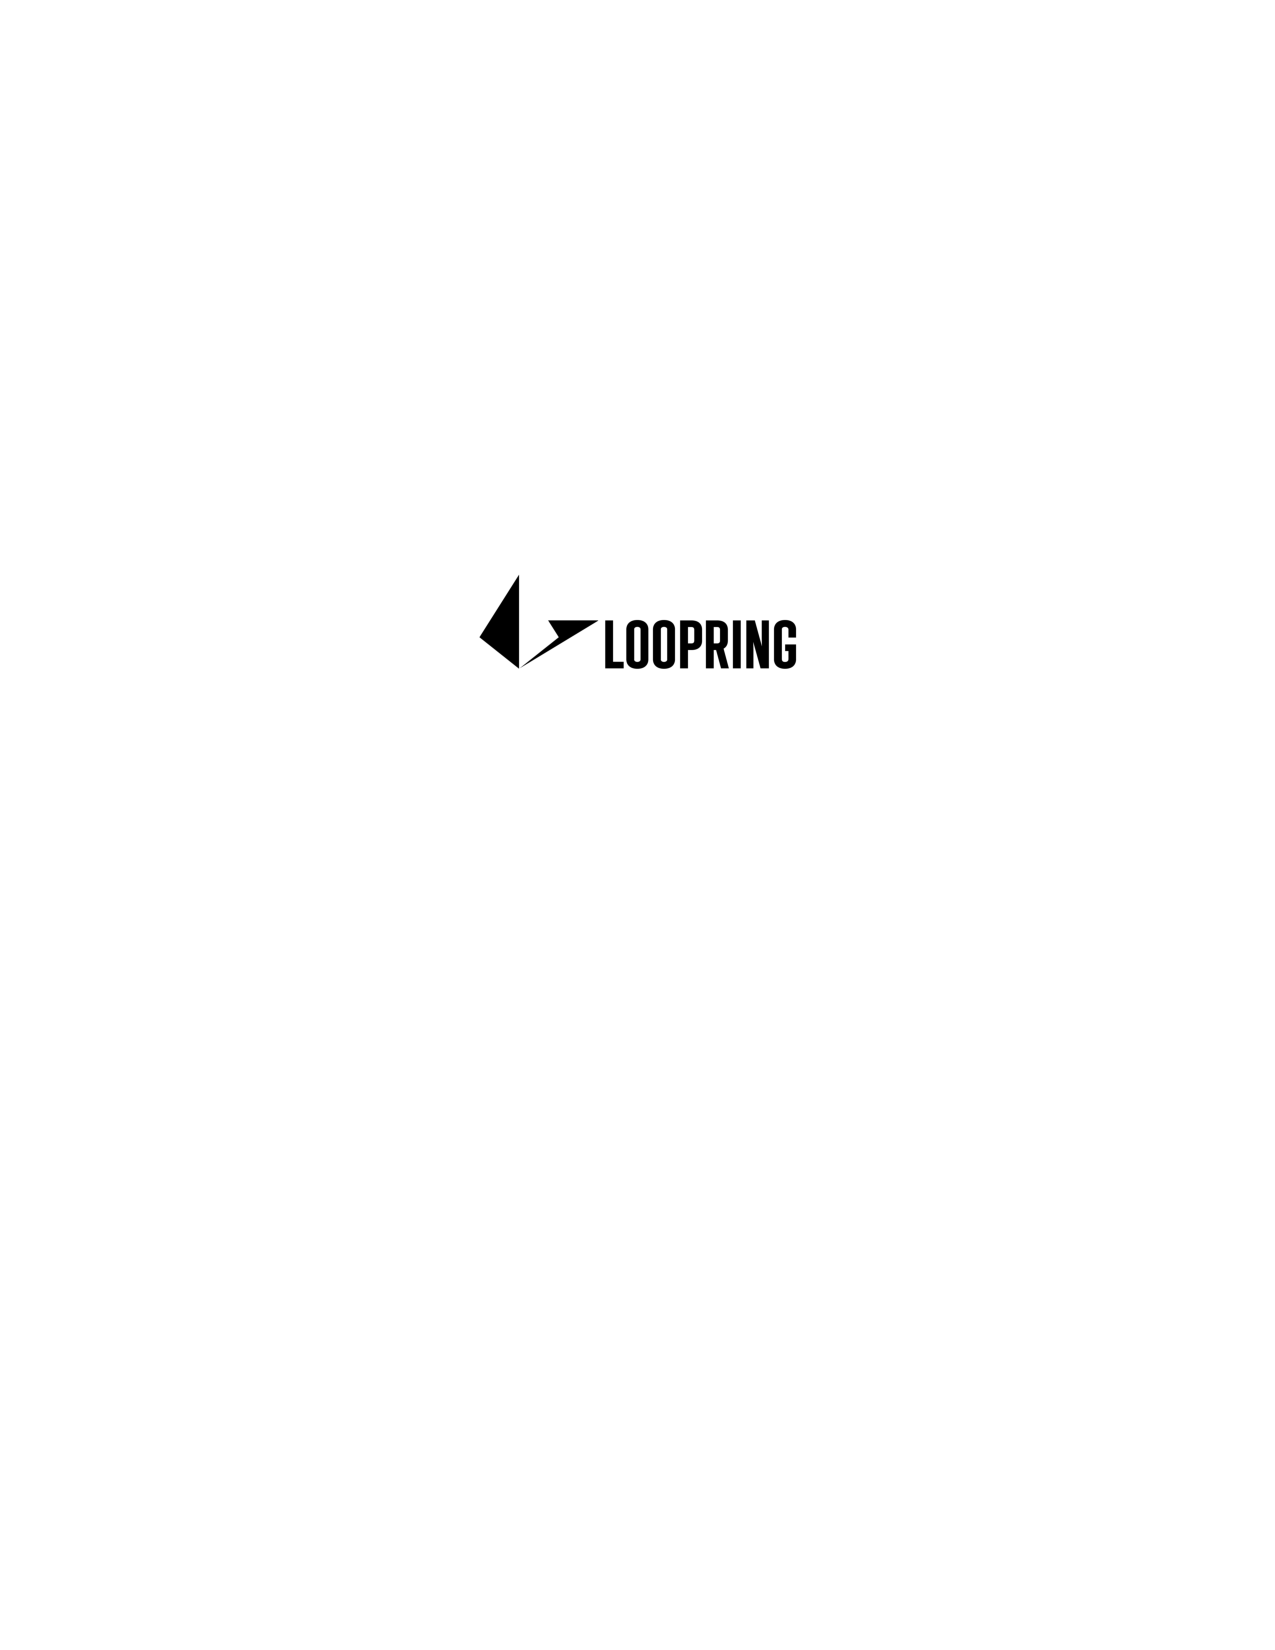
\includepdf[pages=1]{cover}
\hyphenpenalty=750

\title{\textbf{Loopring:}\\\textbf{Ein dezentrales Protokoll zum Tokenhandel}}
\author{
 Daniel Wang\\
  \texttt{daniel@loopring.org}\\
  \and
  	Jay Zhou\\
  	\texttt{jay@loopring.org}\\
  	\and
  	Alex Wang\\
  	\texttt{alex@loopring.org}\\
  	\and
  	Matthew Finestone\\
  	\texttt{matt.finestone@gmail.com}\\ 
  \\
  \texttt{https://loopring.org}
 }

%\makeatletter
%\def\CTEX@section@format{\Large\bfseries}
%\makeatother

\makeatletter
\newenvironment{tablehere}
 {\def\@captype{table}}
 {}

\newenvironment{figurehere}
 {\def\@captype{figure}}
 {}
\makeatother
%
%\newcommand\BackgroundPic{%
%\put(0, 0){%
%\parbox[b][\paperheight]{\paperwidth}{%
%\vfill
%\centering
%\includegraphics[width=\paperwidth, height=\paperheight, %
%%keepaspectratio]{images/background.jpg}%
%]{images/background.jpg}%
%\vfill
%}}}


\begin{document}
%\AddToShipoutPicture{\BackgroundPic}
\maketitle


\begin{abstract}
Loopring ist ein offenes Protokoll, um dezentrale Handelsplattformen zu vernetzen. Mittels öffentlicher Smart Contracts zur Ausführung des Tokenhandels werden Aufträge mehrerer Akteure gesammelt, ausgewertet und unabhängig der Blockchain durchgeführt. Es handelt sich um ein freies, erweiterbares Protokoll und dient als standardisierter Grundbaustein für dezentrale Applikationen (dApps), die den Handel von Token umfassen. Interoperable Standards ermöglichen einen anonymen Handel ohne Dritte. Eine wichtige Verbesserung gegenüber den derzeitigen dezentralen Handelsprotokollen ist die Möglichkeit, dass Aufträge mit anderen, unterschiedlichen Bestellungen gemischt werden können. Dadurch entfällt die Notwendigkeit von Zwei-Token-Handelspaaren und die Liquidität wird drastisch verbessert. Loopring verwendet eine einzigartige und solide Lösung, um ein Front-Running zu verhindern: der unfaire Versuch, Transaktionen schneller als der ursprüngliche Tauschanbieter in einen Block einzureichen. Loopring ist Blockchain-unabhängig und auf jede Blockchain mit Smart-Contract-Funktionalität anwendbar. Derzeit ist Loopring auf Ethereum \cite{buterin2017ethereum} \cite{wood2014ethereum} und Qtum \cite{dai2017smart} nutzbar und befindet sich für NEO \cite{atterlonn2018distributed} in der Entwicklung.
\end{abstract}



\begin{multicols}{2}
\section{Einleitung\label{sec:introduction}}
Mit der Verbreitung von Blockchain-basierten Vermögenswerten hat die Notwendigkeit, diese Güter untereinander auszutauschen, deutlich zugenommen. Da tausende neue Token zusätzlich zu traditionellen Vermögenswerten eingeführt werden, gibt es eine steigende Nachfrage. Unabhängig davon, ob Token zum spekulativen Handel oder für den Einsatz als Utility-Token auf Plattformen erworben werden, ist es essentiell für ein größeres Ökosystem, Krypto-Vermögenswerte untereinander austauschen zu können. Derzeit herrscht eine wachsende Dynamik unter Vermögenswerten \cite{desotocapital}. Um diese zu ermöglichen und Kapital freizugeben, ist nicht nur die Beanspruchung von Eigentum erforderlich, was Blockchains nach wie vor erlauben, sondern auch die Möglichkeit, diese Vermögenswerte frei zu transferieren und zu transformieren.

Der Austausch von Token (Werten) ohne Zwischenhändler ist eine überzeugende Anwendung der Blockchain-Technologie. Dennoch haben sich Krypto-Enthusiasten bislang weitgehend für den Tokenhandel auf traditionellen, zentralisierten Handelsplattformen entschieden. Das Loopring-Protokoll wird benötigt, da - wie Bitcoin \cite{nakamoto2008bitcoin} bereits pflichtgemäß betonte - in Bezug auf elektronisches Geld \enquote{entscheidende Vorteile verloren gehen, wenn noch eine vertrauenswürdige dritte Partei benötigt wird, um doppelte Ausgaben zu vermeiden}. Von daher gehen die Hauptvorteile von dezentralisierten Vermögenswerten verloren, wenn sie über zentrale Handelsplattformen laufen müssen.

Der Handel dezentraler Token an zentralisierten Börsen ist auch aus philosophischer Sicht nicht nachvollziehbar, da das zugrundeliegende Konzept von dezentralisierten Projekten keine Anwendung findet. Es gibt auch zahlreiche praktische Risiken und Einschränkungen bei der Verwendung zentralisierter Tauschbörsen, die nachstehend beschrieben werden. Dezentralisierte Handelsplattformen (DEXs) \cite{schuh2015bitshares} \cite{bancor} \cite{kyber} haben versucht, diese Probleme zu lösen und in vielen Fällen ist es gelungen, Sicherheitsrisiken durch die Verwendung von Blockchains zur Einlagenumschichtung zu mindern. Da die Möglichkeiten dezentraler Handelsplattformen zu einer entscheidenden Infrastruktur für die neue Wirtschaft beitragen, gibt es erheblichen Spielraum für Leistungsverbesserungen. Loopring möchte Module für diese Infrastruktur mittels offenem Protokoll und der Erweiterbarkeit durch dApps bereitstellen.

\section{Aktuelle Handelsplattformen\label{sec:current_exchange_landscape}}

\subsection{Unzulänglichkeiten zentraler Börsen}
Die drei Hauptrisiken zentraler Handelsplattformen sind: 1) Mangel an Sicherheit, 2) Mangel an Transparenz und 3) Mangel an Liquidität.

\textbf{Ein Mangel an Sicherheit} ergibt sich daraus, dass Nutzer typischerweise die Kontrolle über die privaten Schlüssel ihrer Adressen bzw. Konten an eine zentrale Einheit abgeben. Dies setzt Nutzer der Gefahr aus, dass jene zentralisierte Handelsplattformen kriminellen Hackern zum Opfer fallen können. Die Sicherheits- und Hacking-Risiken \cite{coincheckhack}  \cite{mcmillan2014inside}, mit denen sich alle zentralisierten Börsen konfrontiert sehen, sind allgemein bekannt, werden beim Tokenhandel aber oft als gegeben hingenommen. Zentrale Plattformen sind nach wie vor lukrative Ziele für Hackerangriffe, da ihre Server Millionen von Dollar an Vermögenswerten verwalten. Zusätzlich besteht immer die Möglichkeit, dass Programmierern einer Handelsplattform Fehler unterlaufen können, die womöglich zum Verlust von Anlagen führen. Daraus folgt, dass Nutzer nicht die Kontrolle über ihre Vermögenswerte haben, wenn sie an einer zentralisierten Handelsplattform hinterlegt werden.

\textbf{Ein Mangel an Transparenz} führt zum Risiko, dass unseriöse Handelsplattformen unfair agieren. Der Grund liegt darin, dass der Anwender nicht mit seinen tatsächlichen Vermögenswerten handelt, sondern lediglich einen Schuldschein ausgestellt bekommt. Wenn Token in die Geldbörse (Wallet) einer Handelsplattform eingezahlt werden, übernimmt diese die Verwahrung und stellt anstelle der Token einen Schuldschein aus. Alle Tauschgeschäfte finden nunmehr zwischen den Schuldscheinen der Nutzer statt. Um seine Token abzuheben, wird der Schuldschein eingelöst und die Token an eine externe Wallet überwiesen. Während dieses Prozesses besteht ein Mangel an Transparenz und der Austausch kann zum Stillstand kommen, das Konto könnte eingefroren werden, die Handelsplattform könnte pleitegehen usw. Ebenfalls ist es möglich, dass die Vermögen der Anleger in der Zeit der Hinterlegung für andere Zwecke verwendet werden, wie z.B. der Ausleihe an Dritte. Ein Mangel an Transparenz kann Nutzern zusätzliche Kosten verursachen, ohne dass ein Totalverlust der Anlage eintritt, wie etwa höhere Handelsgebühren, Verzögerungen bei hoher Nachfrage, regulatorische Risiken und die Ausführung bevorzugter Aufträge.

\textbf{Der Mangel an Liquidität.} Aus Sicht der Betreiber einer Handelsplattform verhindert eine fragmentierte Liquidität den Einstieg neuer Börsen aufgrund von zwei \enquote{Der Gewinner bekommt alles}-Szenarien. Zum einen gewinnt die Handelsplattform mit der größten Anzahl von Handelspaaren, weil es für die Nutzer vorteilhaft ist, alle ihre Geschäfte an einer Börse abzuwickeln. Zum anderen gewinnt die Handelsplattform mit dem größten Auftragsbuch aufgrund günstiger Ask-Bid-Spannen für jedes Handelspaar. Dies erschwert den Wettbewerb durch Neueinsteiger, da es für sie schwierig ist, eine initiale Liquidität aufzubauen. Infolgedessen haben einige Börsen einen hohen Marktanteil trotz vielfacher Nutzerbeschwerden und teilweise sogar größeren Hackerangriffen. Es ist erwähnenswert, dass schnell wachsende, zentralisierte Börsen zu einem immer größeren Angriffsziel für Hacker werden.

Aus Sicht der Nutzer reduziert eine fragmentierte Liquidität die Benutzerfreundlichkeit erheblich. In einer zentralisierten Börse können Nutzer nur innerhalb der eigenen Liquiditätsspanne und gebunden ans Auftragsbuch zwischen unterstützten Token-Paaren handeln. Um Token A für Token B zu tauschen, müssen sich Nutzer an eine Handelsplattform wenden, welche beide Token unterstützt oder sich an verschiedenen Handelsplattformen registrieren, wobei sie immer persönliche Daten offenlegen. Nutzer müssen häufig vorbereitende Transaktionen durchführen, in der Regel gegen BTC oder ETH, wobei Ask-Bid-Spannen anfallen. Schlussendlich sind die Auftragsbücher möglicherweise nicht groß genug, um den Handel ohne signifikante Preisabweichung abschließen zu können. Selbst wenn die Handelsplattform vorgibt ein großes Volumen zu verarbeiten, gibt es keine Garantie, dass Volumen und Liquidität nicht gefälscht sind \cite{fakevolume}.

Das Ergebnis sind getrennte Liquiditätsmengen und ein fragmentiertes Ökosystem, das dem alten Finanzsystem ähnelt, mit einem bedeutenden und zugleich auf wenige zentrale Handelsplattformen konzentrierten Handelsvolumen. Die globalen Liquiditätsversprechungen der Blockchains bewähren sich nicht im zentralisierten Austausch.

\subsection{Unzulänglichkeiten von dezentralisierten Handelsplattformen}
Dezentrale Handelsplattformen unterscheiden sich von zentralen Tauschbörsen zum Teil dadurch, dass Nutzer die Kontrolle über die privaten Schlüssel ihrer Vermögenswerte behalten, indem sie Transaktionen direkt mit der entsprechenden Blockchain abwickeln. Durch die Nutzung der zugrundeliegenden Trustless-Technologie von Kryptowährungen können viele der oben genannten Sicherheitsrisiken erfolgreich gemindert werden. Probleme bestehen jedoch hinsichtlich Leistung und struktureller Einschränkungen.

Die Liquidität bleibt häufig ein Problem, da Nutzer nach Tauschpartnern bei unterschiedlichen Verfügbarkeiten und Standards suchen müssen. Eine fragmentierte Liquidität tritt dann auf, wenn dezentrale Handelsplattformen oder dApps keine weitläufigen Standards für eine Zusammenarbeit durchsetzen und Aufträge nicht über ein umfangreiches Netzwerk verteilt werden. Die Liquidität von Limit-Auftragsbüchern und insbesondere deren Flexibilität – wie schnell ausgeführte Limit-Aufträge aktualisiert werden – können Handelsstrategien erheblich beeinflussen \cite{limitorderliquidity}. Das Fehlen solcher Standards hat nicht nur zu einer verringerten Liquidität geführt, sondern auch zu einer Reihe von eigenentwickelten, potenziell unsicheren Smart Contracts.

Da Transaktionen auf der Blockchain ausgeführt werden, leiden dezentrale Handelsplattformen an den Einschränkungen der zugrundeliegenden Blockchains: Skalierbarkeit, Verzögerungen bei der Ausführung (Mining) und kostspielige Änderungen von Aufträgen. Blockchain-Auftragsbücher skalieren nur unzureichend, da das Ausführen von Code auf der Blockchain Kosten (Gas) verursacht, wodurch mehrere Auftragsabbrüche unverhältnismäßig teuer werden.

Da die Auftragsbücher der Blockchain öffentlich sind, ist die Transaktion eines neu erstellten Auftrags für die Miner sichtbar, während sie in den nächsten Block geschrieben wird, um im Auftragsbuch zu erscheinen. Diese Verzögerung setzt den Nutzer dem Risiko aus, von anderen überholt und zu seinen Ungunsten unter- bzw. überboten zu werden.

\subsection{Hybride Lösungen}
Aus den obigen Gründen haben rein Blockchain-basierte Handelsplattformen Beschränkungen, die sie gegenüber dem zentralisierten Handel nicht wettbewerbsfähig machen. Es besteht jedoch eine Lösung, um Transaktionen auf der Blockchain, die Geschwindigkeit von zentralen Handelsplattformen und die Tauschflexibilität zu vereinen. Protokolle wie Loopring und 0x \cite{warren20170x} erweitern eine Lösung der On-Chain-Abwicklung mit Off-Chain-Bestellmanagement. Dieses Konzept agiert mit offenen Smart Contracts, vermeidet Skalierbarkeitsbeschränkungen, indem es mehrere Funktionen unabhängig der Blockchain ausführt und den Schnittstellen ausreichende Flexibilität in der Erfüllung von Netzwerkentscheidungen einräumt. Nachteile bleiben jedoch auch im Hybridmodell bestehen \cite{costofdecent}. Das Loopring-Protokoll stellt mit dieser Abhandlung sinnvolle Lösungsansätze für eine hybride Technik vor.

\section{Loopring-Protokoll\label{sec:loopring_protocol}}
Loopring ist keine dezentrale Handelsplattform, sondern ein modulares Protokoll zum Aufbau von DEXs auf mehreren Blockchains. Loopring teilt die Bausteine einer traditionellen Handelsplattform auf und setzt stattdessen auf eine Kombination aus offenen Smart Contracts und dezentralen Akteuren. Zu den Bestandteilen im Netzwerk zählen Wallets, Netzwerkknoten, Liquidität-teilende Blockchains, Browser für Auftragsbücher, Ring-Miner und Dienste zur Tokenisierung von Vermögenswerten. Bevor darauf näher eingegangen wird, sollte man zuerst die Loopring-Aufträge verstehen.

\subsection{Bestellkreislauf\label{sec:order_ring}}
Loopring-Aufträge werden in einem multidimensionalen Bestellmodell (Unidirectional Order Model) \cite{coinport2014udom} verarbeitet. Das UDOM stellt Aufträge zum Tokentausch aus, \verb|amountS|/\verb|amountB|, (Menge zu verkaufen/kaufen) anstelle von Ask-Bid-Preisen. Da jede Bestellung nur eine Austauschrate zwischen zwei Token ist, ist eine tragende Rolle des Protokolls das Mischen und Abgleichen mehrerer Bestellungen im Handelskreislauf. Durch den Einsatz von bis zu 16 Aufträgen anstelle eines einzelnen Handelspaars steigt die Liquidität rapide an und bietet Potenzial zur Preisverbesserung.

\begin{center}
\begin{figurehere}
\centering
\tikzstyle{block} = [draw, fill=blue!20, rectangle, 
    minimum height=3em, minimum width=6em]
\tikzstyle{sum} = [draw, fill=blue!20, circle, node distance=1cm]
\tikzstyle{input} = [coordinate]
\tikzstyle{output} = [coordinate]
\tikzstyle{pinstyle} = [pin edge={to-,thin,black}]

\begin{tikzpicture}[
    auto, 
    node distance=2cm,
    >=latex',
    font=\bfseries\footnotesize\sffamily,
    order/.style={
		scale=0.7,
		rectangle,
		rounded corners,
		draw=black, 
		text centered,
%		text width=5cm,
		minimum height=12mm,
		fill=white
	},
	label/.style={
		scale=0.7
	}
  ]
    % We start by placing the blocks

  \node [order] (order2) 
 {%
 \begin{tabular}{l}
  \textbf{AUFTRAG \#2}\\
  \textbf{Inhaber: Y}\\
  \textbf{Menge V: 9B}\\
  \textbf{Menge K: 12C}
 \end{tabular}
 };
 
  \node [order, below of=order2, xshift=-3.5cm] (order1) 
 {%
 \begin{tabular}{l}
  \textbf{AUFTRAG \#1}\\
  \textbf{Inhaber: X}\\
  \textbf{Menge V: 10000A}\\
  \textbf{Menge K: 2B}
 \end{tabular}
 };
 
 
  \node [order, below of=order2, xshift=3.5cm] (order3) 
 {%
 \begin{tabular}{l}
  \textbf{AUFTRAG \#3}\\
  \textbf{Inhaber: Z}\\
  \textbf{Menge V: 100C}\\
  \textbf{Menge K: 160A}
 \end{tabular}
 };
 
 \draw [draw,->] (order1) -- node [label] {\textbf{7898A}} (order3);
 \draw [draw,->] (order2) -| node [label, xshift=-1.8cm] {\textbf{8B}} (order1);
 \draw [draw,->] (order3) |- node [label, xshift=1cm, yshift=0.24cm] {\textbf{98C}} (order2);

\end{tikzpicture}

\caption{Auftragsring von drei Bestellungen}
\label{fig:ring}
\end{figurehere}
\end{center}


Die obige Abbildung zeigt einen Handelskreislauf mit drei Aufträgen. Jeder Token, der zum Verkauf steht (\verb|tokenS|), wird in einem anderen Auftrag zum Kauf (\verb|tokenB|) angefragt. Es entsteht ein Ring, der es jeder Bestellung erlaubt, ihre gewünschten Token zu tauschen ohne auf ein weiteres Handelspaar angewiesen zu sein. Herkömmliche Abwicklungen von Auftragspaaren können dennoch ausgeführt werden, was jedoch einen Sonderfall im Bestellkreislauf darstellt.

\begin{definition}[Bestellkreislauf] $C_{0}$, $C_{1}$, $\cdots$, $C_{n-1}$ sind $n$ unterschiedliche Token, $O_{0\rightarrow 1}$, $\cdots$, $O_{i\rightarrow i\oplus 1}$, $\cdots$, $O_{n-1 \rightarrow 0}$ sind $n$ Aufträge. Diese Aufträge können einen Bestellkreislauf formen:
$$O_{0\rightarrow 1} \rightarrow \cdots \rightarrow O_{i\rightarrow i\oplus 1} \rightarrow \cdots \rightarrow O_{n-1\rightarrow 0} \text{, }$$
wobei $n$ die Länge des Auftragsrings ist, und $i\oplus 1 \equiv i+1 \mod n$.
\end{definition}

Ein Auftragsring ist gültig, wenn alle Token-Transaktionen zu einem Wechselkurs ausgeführt werden können, der gleich oder besser ist als der ursprünglich vom Nutzer festgelegte Kurs. Um die Gültigkeit des Handels zu überprüfen, beziehen Smart Contracts des Loopring-Protokolls den Bestellkreislauf von sogenannten Ring-Minern, wobei das Produkt der ursprünglichen Wechselkurse aller Bestellungen gleich oder größer als 1 sein muss.

Nehmen wir an, Alice und Bob wollen ihren Token \verb|A| und \verb|B| tauschen. Alice hat 15 Token \verb|A| und möchte 4 Token \verb|B| erhalten. Bob hat 10 Token \verb|B| und möchte 30 Token \verb|A|.

Wer kauft und wer verkauft? Dies hängt allein von dem Token ab, welcher als Referenz herangezogen wird. Wenn Token \verb|A| die Referenz ist, dann kauft Alice Token \verb|B| für den Preis von ${15 \over 4} = 3.75$\verb|A|, während Bob 10 Token \verb|B| für den Preis von ${30 \over 10} = 3.00$\verb|A| verkauft. Für den Fall, dass Token \verb|B| die Referenz ist, verkauft Alice 15 Token \verb|A| für den Preis von ${4\over 15}=0.26666667$\verb|B| und Bob kauft 10 Token \verb|A| für den Preis von ${10 \over 30}=0.33333334$\verb|B|. Von daher können Käufer und Verkäufer willkürlich gewählt werden.

Im ersten Fall ist Alice bereit einen höheren Preis ($3.75$\verb|A|) zu bezahlen als Bob für seine Token verlangen würde ($3.00$\verb|A|), wobei im zweiten Fall Bob bereit ist einen höheren Preis ($0.33333334$\verb|B|) für Alice's Token zu geben ($0.26666667$\verb|B|). Es ist offensichtlich, dass ein Handel möglich ist, wann immer der Käufer bereit ist, einen gleichen oder höheren Preis als den des Verkäufers zu zahlen.

\begin{equation}
{{15\over 4} \over {30\over 10}} = {{10\over 30} \over {4\over 15}}={15 \over 4} \cdot {10 \over 30} = 1.25 > 1
\end{equation}

Damit ein Satz von $n$ Aufträgen ganz oder teilweise erfüllt werden kann, müssen wir wissen, ob das Produkt eines jeden Wechselkurses als Kaufauftrag zu einer Zahl größer oder gleich 1 führt. Wenn ja, können alle $n$ Aufträge entweder teilweise oder vollständig abgewickelt werden.

Wir ziehen eine dritte Partei – Charlie – hinzu, so dass Alice $x_1$ Token \verb|A| verkaufen und dafür $y_1$ Token \verb|B| erhalten möchte, Bob will $x_2$ Token \verb|B| geben und dafür $y_2$ Token \verb|C| erhalten und Charlie möchte $x_3$ Token \verb|C| geben und dafür $y_3$ Token \verb|A| erhalten. Die erforderlichen Token sind vorhanden und der Handel ist möglich, wenn:

\begin{equation}
{{x_1 \cdot x_2 \cdot x_3 \over y_1 \cdot y_2 \cdot y_3} \geq 1}
\end{equation}


Siehe Punkt \ref{anatomy} für detaillierte Informationen über Loopring-Aufträge.



\section{Bestandteile des Ökosystems\label{sec:ecosystem}}
Die folgenden Parteien stellen gemeinsam alle Funktionalitäten, die auch ein zentralisierter Austausch bietet.

\begin{itemize}

\item \textbf{Wallets}: Ein gewöhnlicher Kontoservice bzw. Bedienoberfläche, der Nutzern den Zugriff auf ihre Token und eine Möglichkeit zum Senden von Aufträgen an das Loopring-Netzwerk bietet. Wallets werden durch das Teilen von Gebühren mit Ring-Minern angespornt, Aufträge zu erstellen (siehe Abschnitt \ref{sec:token}). Mit der Absicht, dass die Zukunft des Handels durch die Sicherheit von individuellen Wallets erfolgt, hat die Verbindung dieser Liquiditätsmengen durch unser Protokoll oberste Priorität.

\item \textbf{Konsortium von Liquidität fördernden Blockchains und Netzwerkknoten}: Ein Netzwerk zur Auftrags- und Liquiditätssteigerung. Wenn einzelne Netzwerkknoten die Loopring-Vermittlungssoftware anwenden, können sie einem bereits existierenden Netzwerk beitreten und die Liquidität auf Grundlage der vereinigten Blockchain-Interessengemeinschaft vorantreiben. Die erste vereinigte Blockchain, die wir erschaffen, hat nahezu eine Auftragsteilung in Echtzeit (1-2 Sekunden-Blöcke) und setzt neue Maßstäbe, um ein schnelleres Herunterladen durch neue Netzwerkknoten zu ermöglichen.

\item \textbf{Netzwerkknoten/Ring-Miner}: Netzwerkknoten sind Schnittstellen, die Aufträge von Wallets oder anderen Knoten erhalten, öffentliche Auftragsbücher und Auftragshistorien verwalten und optional Aufträge zu anderen Schnittstellen übertragen (via beliebigem Off-Chain-Medium). Ring-Mining ist eine Option für Schnittstellen, keine Anforderung. Es ist rechenintensiv und erfolgt vollständig off-chain. Netzwerkknoten, welche diese Funktion aktiviert haben, werden \enquote{Ring-Miner} genannt und Bestellkreisläufe ermöglichen, indem sie unterschiedliche Aufträge zusammenführen. Netzwerkknoten können frei wählen (1) wie sie sich untereinander verständigen, (2) wie sie ihre Auftragsbücher aufbauen und (3) wie sie Auftragsringe abbauen (Mining-Algorithmen).

\item \textbf{Loopring Protocol Smart Contracts (LPSC)}: Ein Zusammenschluss öffentlicher Smart Contracts, der Auftragsringe von Ring-Minern überprüft, Token im Namen der Nutzer transferiert, den Ring-Minern und Wallets Anreize durch Gebühren bietet und Ereignisse kommuniziert. Schnittstellen bzw. Auftragsbuch-Browser orientieren sich an den Informationen, um ihre Auftragsbücher und Handelshistorie aktuell zu halten. Siehe Anhang \ref{app:protocol_ethereum} für Details.

\item \textbf{Asset Tokenization Services (ATS)}: Angebote zur Tokenisierung, die den Tausch von nicht über Loopring handelbaren Gütern ermöglichen. Diese bestehen aus zentralen Diensten, welche von vertrauenswürdigen Unternehmen oder Organisationen bereitgestellt werden. Nutzer hinterlegen Werte (physisch, Fiat, Token anderer Blockchains) und bekommen Token ausgestellt, die zukünftig wieder eingetauscht werden können. Loopring ist kein Blockchain-übergreifendes Handelsprotokoll (bis eine geeignete Lösung existiert), jedoch ermöglicht ATS sowohl den Handel von ERC20-Token \cite{ERC20} mit physikalischen Gütern als auch mit Vermögenswerten anderer Blockchains.

\end{itemize}


\section{Handelsprozess\label{sec:process}}



\begin{enumerate} 


\item \textbf{Protokollautorisierung}: In Abbildung \ref{fig:process} autorisiert Inhaber \verb|Y|, der Token handeln möchte, den LPSC \verb|amountS| seiner Token \verb|B| zu verwalten um sie zu verkaufen. Der LPSC sperrt nicht die Token des Inhabers und es steht dem Inhaber frei die Token zu nutzen, solange der Auftrag bearbeitet wird.

\item \textbf{Auftragserstellung}: Der aktuelle Preis und das Auftragsbuch für den Token \verb|B| gegen Token \verb|C| wird von Netzwerkknoten oder anderen Agenten wie Auftragsbuch-Browsern zur Verfügung gestellt, die mit dem Netzwerk verbunden sind. Inhaber \verb|Y| erstellt einen Auftrag (Limit-Auftrag), indem er \verb|amountS| und \verb|amountB| sowie andere Parameter mithilfe einer eingebauten Wallet-Oberfläche festlegt. Der LRx-Betrag kann dem Auftrag als Gebühr für die Ring-Miner hinzugefügt werden. Höhere LRx-Gebühren bedeuten eine höhere Chance früher von Ring-Minern bearbeitet zu werden. Der Hash des Auftrags wird durch den privaten Schlüssel des Inhabers \verb|Y| signiert.

\item \textbf{Auftragsverteilung}: Das Wallet überträgt den Auftrag und seine Signatur an eine oder mehrere Netzwerkknoten. Diese aktualisieren ihr Auftragsbuch. Das Protokoll schreibt nicht vor, wie diese Auftragsbücher auszusehen haben z.B. dass der erste Auftrag bevorzugt abgewickelt werden muss. Stattdessen sind Knoten frei in der Gestaltung ihres Auftragsbuches.

\item \textbf{Liquidität teilen}: Netzwerkknoten verteilen den Auftrag mittels beliebigem Medium an andere Schnittstellen. Auch hier sind Netzwerkknoten flexibel, ob und wie sie interagieren. Um ein gewisses Maß an Netzwerkkonnektivität zu gewährleisten, gibt es eine integrierte Liquiditätsteilung unter den Schnittstellen auf Grundlage einer vereinigenden Blockchain. Wie im vorherigen Abschnitt erwähnt, ist dieses Netzwerk auf Geschwindigkeit und Inklusivität optimiert.

\begin{center}
\begin{figurehere}
\centering
\tikzstyle{block} = [draw, fill=blue!20, rectangle, 
    minimum height=3em, minimum width=6em]
\tikzstyle{sum} = [draw, fill=blue!20, circle, node distance=1cm]
\tikzstyle{input} = [coordinate]
\tikzstyle{output} = [coordinate]
\tikzstyle{pinstyle} = [pin edge={to-,thin,black}]

\begin{tikzpicture}[
    auto, 
    scale=0.7,
    node distance=2cm,
    >=latex',
    font=\bfseries\footnotesize\sffamily,
    order/.style={
		rectangle,
		scale=0.7,
		rounded corners,
		draw=black, 
		text centered,
%		text width=5cm,
		minimum height=12mm,
		minimum width=30mm,
		fill=white
	},
	role/.style={
		circle,
		scale=0.7,
		draw=black, 
		text centered,
%		text width=5cm,
		minimum height=12mm,
		minimum width=12mm,
		fill=white
	},
	steps/.style={
		circle,
		scale=0.7,
		draw=black, 
		text centered,
%		text width=5cm,
%		minimum height=12mm,
%		minimum width=12mm,
		fill=black,
		text=white
	},
	account/.style={
		circle,
		scale=0.7,
		draw=black, 
		text centered,
%		text width=5cm,
		minimum height=16mm,
		minimum width=16mm,
		fill=white
	},
	label/.style={
	  scale=0.7
    }
  ]

 
 \node [role] (user1)  {Inhaber X};
 \node [role, below of=user1] (user2)  {Inhaber Y};
 \node [role, below of=user2] (user3)  {Inhaber Z};
 \node [role, below of=user3, fill=gray!20] (relay1)  {Anfrage M};
 \node [role, below of=relay1, fill=gray!20] (relay2)  {Anfrage N};

 
 \node [order, left of=user1, xshift=-1cm] (order1) 
 {%
 \begin{tabular}{l}
  \textbf{AUFTRAG 1}\\
  \textbf{Inhaber: X}\\
  \textbf{Menge V: 10000 A}\\
  \textbf{Menge K: 2 B}
 \end{tabular}
 };
 
 \draw [draw, ->]  (user1) -- (order1) [label]{};
 \draw [bend right,->] (order1) to node [auto, scale=0.7] {} (relay1);
 \draw [bend right,->] (order1) to node [auto, scale=0.7] {} (relay2);
% \draw [draw, ->]  (order1) |- (relay1) [label]{};
% \draw [draw, ->]  (order1) |- (relay2) [label]{};
 
 \node [order,left of=user2, xshift=-1.5cm] (order2) 
 {%
 \begin{tabular}{l}
  \textbf{AUFTRAG 2}\\
  \textbf{Inhaber: Y}\\
  \textbf{Menge V: 9  B}\\
  \textbf{Menge K: 12 C}
 \end{tabular}
 };
 \draw [draw, ->]  (user2) -- (order2) [label]{};
 \draw [bend right,->] (order2) to node [auto, scale=0.7] {} (relay1);
 \draw [bend right,->] (order2) to node [auto, scale=0.7] {} (relay2);
% \draw [draw, ->]  (order2) |- (relay1) [label]{};
% \draw [draw, ->]  (order2) |- (relay2) [label]{};
% 
\node [order, left of=user3, xshift=-2cm] (order3) 
 {%
 \begin{tabular}{l}
  \textbf{AUFTRAG 3}\\
  \textbf{Inhaber: Z}\\
  \textbf{Menge V: 100 C}\\
  \textbf{Menge K: 160 A}
 \end{tabular}
 };
 \draw [draw, ->]  (user3) -- (order3) [label]{};
 \draw [bend right,->] (order3) to node [auto, scale=0.7] {} (relay1);
 \draw [bend right,->] (order3) to node [auto, scale=0.7] {} (relay2);
% \draw [draw, ->]  (order3) |- (relay1) [label]{};
% \draw [draw, ->]  (order3) |- (relay2) [label]{};
 
% // The Ring
\node [order, 
yshift=-1.5cm,
xshift=-2.75cm,
below of=relay2,
fill=gray!10,
minimum width=4.2cm,
minimum height=5cm] (ring) {};


\node [order, dashed, below of=relay2,yshift=-0.2cm,xshift=-2.5cm] (order11) 
 {%
 \begin{tabular}{l}
  \textbf{AUFTRAG 1}\\
  \textbf{Inhaber: X}\\
  \textbf{Menge V: 10000 A}\\
  \textbf{Menge K: 2 B}
 \end{tabular}
 };
 \node [order, dashed,below of=order11,xshift=-0.25cm,yshift=0.7cm] (order21) 
 {%
 \begin{tabular}{l}
  \textbf{AUFTRAG 2}\\
  \textbf{Inhaber: Y}\\
  \textbf{Menge V: 9  B}\\
  \textbf{Menge K: 12 C}
 \end{tabular}
 };
\node [order, dashed,below of=order21,xshift=-0.25cm,yshift=0.7cm] (order31) 
 {%
 \begin{tabular}{l}
  \textbf{AUFTRAG 3}\\
  \textbf{Inhaber: Z}\\
  \textbf{Menge V: 100 C}\\
  \textbf{Menge K: 160 A}
 \end{tabular}
 };
 
 % // The blockchain
\node [
rectangle,
fill=gray!20, 
right of=user1,
yshift=-4.5cm,
xshift=0.1cm,
scale=0.7,
minimum width=3.2cm,
minimum height=15.6cm] (blockchain) {\parbox[b][15cm]{1.3cm}{Blockchain}};
% blockchain accounts
  \node [account, right of=user1, xshift=1cm] (account1)  {Wallet X};
  \node [account, right of=user2, xshift=1cm] (account2)  {Wallet Y};
  \node [account, right of=user3, xshift=1cm] (account3)  {Wallet Z};
  \node [account, right of=relay1, xshift=1cm] (account4)  {Wallet M};
  \node [account, right of=relay2, xshift=1cm] (account5)  {Wallet N};
  \node [account, double, below of=account5, yshift=-1.5cm] (psc)  {LPSC};
  
 \draw [draw, ->]  (user1) -- (account1) [label]{};
 \draw [draw, ->]  (user2) -- (account2) [label]{};
 \draw [draw, ->]  (user3) -- (account3) [label]{};
% \draw [draw, ->]  (relay1) -- (account4) [label]{};
% \draw [draw, ->]  (relay2) -- (account5) [label]{};
 \draw [draw, double, thick]  (relay1) to node [auto, scale=0.7] {teilen Liquidität}  (relay2) [label]{};
% \draw [draw, ->]  (relay1) -- (ring) [label]{};
 \draw [draw, ->]  (relay2) to node [auto, scale=0.7, xshift=-1.8cm, yshift=0.3cm] {Ring-Mining}  (ring) [label]{};
 \draw [draw, ->]  (ring) to node [auto, scale=0.7] {Ring einreichen} (psc) [label]{};
 
 \draw [bend left,->] (account1) to node [auto, scale=0.7] {\textbf{7898 A}} (account3);
 \draw [bend left,->] (account2) to node [auto, scale=0.7] {\textbf{8 B}} (account1);
 \draw [bend left,->] (account3) to node [auto, scale=0.7] {\textbf{98 C}} (account2);
 
 \draw [bend left,->, dashed] (account1) to node [auto, scale=0.7] {} (account5);
 \draw [bend left,->, dashed] (account2) to node [auto, scale=0.7] {} (account5);
 \draw [bend left,->, dashed] (account3) to node [auto, scale=0.7, xshift=.5cm] {\textbf{Gebühr}} (account5);
  
  
% \draw [draw,->] (order1) -- node [label] {\textbf{7898 A}} (order3);
% \draw [draw,->] (order2) -| node [label, xshift=-1.8cm] {\textbf{8 B}} (order1);
% \draw [draw,->] (order3) |- node [label, xshift=1cm, yshift=0.24cm] {\textbf{98 C}} (order2);

\node [steps, right of=user2, xshift=-0.6cm] () {1};
\node [steps, left of=user2, xshift=0.8cm] () {2};
\node [steps, left of=relay2, xshift=0.3cm, yshift=1cm] () {3};
\node [steps, left of=relay1, xshift=3.3cm, yshift=-1.6cm] () {4};
\node [steps, below of=relay2, xshift=-0.2cm, yshift=0.4cm] () {5};
\node [steps, right of=account3, xshift=-0.6cm] (step5) {6};

 \draw [bend right, ->]  (psc) to node [auto, scale=0.7, xshift=0.5cm] {Ausführung} (step5) [label]{};
 
\end{tikzpicture}

\caption{Handelsprozess von Loopring}
\label{fig:process}
\end{figurehere}
\end{center}

\item \textbf{Ring-Mining (Auftragsabgleich)}: Ring-Miner versuchen den Auftrag vollständig oder teilweise zu dem geforderten Preis oder besser zu erfüllen, indem sie ihn mit mehreren anderen Aufträgen abgleichen. Ring-Mining ist der Hauptfaktor, durch den das Protokoll eine hohe Liquidität zu jedem Paar bereitstellen kann. Wenn der ausgeführte Kurs besser ist als der von Nutzer Y angegebene Wert, wird die Marge unter allen Aufträgen im Bestellkreislauf aufgeteilt. Als Belohnung kann der Ring-Miner zwischen einer einfachen LRx-Gebühr oder der Beteiligung an der Marge (Margin Split) wählen, wobei er in diesem Fall die LRx-Gebühr zurückzahlen muss.

\item \textbf{Überprüfung \& Abrechnung}: Der LPSC erhält den Auftragsring. Er führt mehrere Überprüfungen durch, um die vom Ring-Miner gelieferten Daten zu verifizieren und stellt fest, ob der Bestellkreislauf ganz oder teilweise erfüllt werden kann (abhängig von der Füllrate der Ring-Aufträge und den Token im Nutzerkonto). Wenn alle Überprüfungen erfolgreich sind, überträgt der Smart Contract die Token automatisch an die Nutzer und zahlt gleichzeitig die Ring-Miner und Wallet-Gebühren. Wenn das Kontoguthaben des Inhabers \verb|Y| vom LPSC als nicht ausreicht erkannt wird, wird dieser Auftrag verkleinert: Ein reduzierter Auftrag wird automatisch auf die ursprüngliche Größe skaliert, sobald ausreichende Mittel dem Konto hinzugefügt werden, anders als ein Abbruch, der nur manuell in eine Richtung verläuft und nicht rückgängig gemacht werden kann.

\end{enumerate}





%
%\end{multicols}
%
%\begin{center}
%\begin{figurehere}
%\includegraphics[height=8cm]{images/en_protocol.png}
%\caption{Loopring Trading Process}
%\label{fig: Loopringrotocol}
%\end{figurehere}
%\end{center}
%
%\begin{multicols}{2}

\section{Operative Flexibilität\label{sec:business_model}}
Es ist wichtig zu beachten, dass der freie Loopring-Standard den Teilnehmern eine große Flexibilität in der Ausführung ermöglicht. Akteuren steht es frei, neue Geschäftsmodelle zu implementieren und den Nutzern einen Mehrwert zu bieten, indem sie LRx-Gebühren für das Volumen oder andere Maße im Prozess verdienen (wenn sie dies wünschen). Das Ökosystem ist modular aufgebaut und soll die Teilnahme einer Vielzahl von Anwendungen unterstützen.

\subsection{Auftragsbuch\label{sec:order_book}}
Netzwerkknoten können ihre Auftragsbücher auf verschiedene Arten gestalten, um die Bestellungen der Nutzer anzuzeigen und abzugleichen. Eine erste Implementierung unseres eigenen Auftragsbuches folgt einem \enquote{Over the counter}-Modell (OTC), bei dem Limit-Aufträge nur auf Basis des Preises positioniert werden. Zeitstempel von Aufträgen haben demnach keine Auswirkungen auf das Auftragsbuch, jedoch steht es den Netzwerkknoten frei, ihr Auftragsbuch so zu gestalten, dass Zeitstempel wie ein typisches Auftragsbuch einer zentralisierten Handelsplattform ebenso berücksichtigt werden. Wenn ein Knoten diese Art von Auftragsbuch anbieten möchte, kann er ein Wallet vernetzen und dessen Aufträge alleinig über seine Schnittstelle abwickeln, um sie zeitabhängig zu verteilen. Derartige Konfigurationen sind möglich.

Während andere DEX-Protokolle Anforderungen an ein Tokenguthaben seitens der Netzwerkknoten stellen, damit diese Taker-Aufträge veranlassen können, müssen Loopring-Schnittstellen nur passende Aufträge finden um einen Handel einzuleiten. Dieser Schritt bedarf keiner eigenen Token.

\subsection{Liquiditätsteilung\label{sec:liquidity_sharing}}
Netzwerkknoten können frei entscheiden, wie sie Liquidität (Aufträge) miteinander teilen. Unsere Konsortium-Blockchain ist nur eine Lösung um dies zu erreichen. Dem Ökosystem steht es frei, sich nach eigenem Belieben zu vernetzen und zu kommunizieren. Knoten können sich nicht nur der Blockchain eines Konsortiums anschließen, sondern auch ihre eigene Blockchain mit Regeln und Besonderheiten entwerfen. Sie können ebenfalls alleine agieren, wie mit der zeitbasierten Wallet-Implementierung beschrieben. Wenngleich unterschiedliche Geschäftsmodelle besondere Verteilstrategien berücksichtigen und die Vergabe von Gebühren beliebig gestalten können, existieren offensichtliche Vorteile in der Kommunikation mit anderen Schnittstellen hinsichtlich Netzwerkeffekte.

\section{Spezifikation des Protokolls\label{sec:protocol}}

\subsection{Anatomie eines Auftrags\label{anatomy}}
Ein Auftrag ist ein Datenpaket, das die Absicht des Nutzers zum Handel ausdrückt. Ein Loopring-Auftrag wird mithilfe des multidimensionalen Bestellmodells (UDOM) wie folgt definiert:

\begin{verbatim}
  message Order {
    address protocol;
    address owner;
    address tokenS;
    address tokenB;
    uint256 amountS;
    uint256 amountB;
    unit256 lrcFee
    unit256 validSince; // Seconds since epoch
    unit256 validUntil; // Seconds since epoch
    uint8   marginSplitPercentage;  // [1-100]
    bool    buyNoMoreThanAmountB;
    uint256 walletId;
    // Dual-Authoring address
    address authAddr;
   	// v, r, s are parts of the signature
    uint8   v;       
    bytes32 r;
    bytes32 s;
    // Dual-Authoring private-key,
    // not used for calculating order's hash,
    // thus it is NOT signed.
    string  authKey;          
  }
\end{verbatim}

Um den Ursprung des Auftrags sicherzustellen, wird er gegen den Hash seiner Parameter mittels privatem Schlüssel des Nutzers signiert (nicht \verb|authAddr|). Der \verb|authAddr| Parameter wird für das Signieren des zugehörigen Auftragsrings verwendet, um ein Front-Running zu verhindern. Weitere Informationen finden Sie in Abschnitt \ref{sec:dual_authoring}. Die Signatur wird durch die Felder \verb|v|, \verb|r|, und \verb|s| repräsentiert und zusammen mit den Auftragsparametern über das Netzwerk gesendet. Dies garantiert, dass die Bestellung während ihrer gesamten Lebensdauer unveränderbar bleibt. Auch wenn sich der Auftrag niemals ändert, kann das Protokoll seinen aktuellen Status basierend auf dem Guthaben seiner Adresse zusammen mit anderen Variablen berechnen.

UDOM enthält keinen Preis (der naturgemäß eine Gleitkommazahl sein muss), sondern verwendet stattdessen den Begriff \verb|rate| oder $r$, welcher als \verb|amountS|/\verb|amountB| (Menge V/K) ausgedrückt wird. \verb|rate| ist keine Gleitkommazahl, sondern eine Form, die nur mit anderen unsignierten ganzen Zahlen bei Bedarf ausgewertet wird, um alle zwischenzeitlichen Ergebnisse als ganze Zahlen während der Kalkulation beizubehalten.

\subsubsection{Kaufbeträge}

Wenn ein Ring-Miner Aufträge abgleicht, besteht die Möglichkeit, dass ein besserer Wechselkurs erzielbar ist. Dies erlaubt es dem Nutzer mehr \verb|tokenB| zu erhalten als die Summe, die mittels \verb|amountB| spezifiziert wurde. Sollte jedoch \verb|buyNoMoreThanAmountB| auf \verb|True| gesetzt sein, stellt das Protokoll sicher, dass der Nutzer nicht mehr als \verb|amountB| von \verb|tokenB| erhält. Somit bestimmt UDOM's \verb|buyNoMoreThantokenB| Parameter, wann ein Auftrag als vollständig erfüllt angesehen wird. \verb|buyNoMoreThantokenB| gilt als eine Obergrenze für entweder \verb|amountS| oder \verb|amountB| und erlaubt es dem Nutzer, detailliertere Handelsabsichten auszudrücken als traditionelle Kauf- und Verkaufsaufträge.

Beispiel: mit \verb|amountS| = 10 und \verb|amountB| = 2, wäre der Kurs $r$ = 10/2 = 5. Also möchte der Nutzer 5 \verb|tokenS| für jeden \verb|tokenB|. Der Ring-Miner vergleicht und findet einen Auftrag mit dem Kurs 4, welcher es dem Nutzer erlaubt, 2.5 \verb|tokenB| anstatt 2 zu erhalten. Möchte der Nutzer jedoch nur 2 \verb|tokenB| und hat den Parameter \verb|buyNoMoreThanAmountB| auf \verb|True| gesetzt, wird die Transaktion mit dem Kurs 4 ausgeführt, wodurch er 4 \verb|tokenS| für jeden \verb|tokenB| erhält und folgerichtig 2 \verb|tokenS| spart. Es muss beachtet werden, dass hierbei Mining-Gebühren nicht berücksichtigt werden (siehe Abschnitt \ref{sec:fee_model}).

Wenn wir Folgendes verwenden


\begin{verbatim}
	      Order(amountS,tokenS,
	            amountB,tokenB,
	            buyNoMoreThantokenB)
\end{verbatim}

um einen Auftrag vereinfacht darzustellen, können populäre Kauf-/Verkauf-Modelle für ETH/USD-Märkte an einer traditionellen Handelsplattform den unten abgebildeten ersten und dritten Auftrag ausdrücken, jedoch nicht die anderen beiden:

\begin{enumerate}
	\item Verkaufe 10 ETH für 300 USD/ETH. Dieser Auftrag kann wie folgt dargestellt werden: \verb|Order(10, ETH, 3000, USD, False)|.
	\item Verkaufe ETH für 300 USD/ETH um 3000 USD zu erhalten. Dieser Auftrag kann wie folgt dargestellt werden: \verb|Order(10, ETH, 3000, USD, True)|.
	\item Kaufe 10 ETH für 300 USD/ETH. Dieser Auftrag kann wie folgt dargestellt werden: \verb|Order(3000, USD, 10, ETH, True)|.
	\item Gebe 3000 USD aus, um so viel ETH wie möglich zu kaufen zum Preis von 300 USD/ETH. Dieser Auftrag kann wie folgt dargestellt werden: \verb|Order(3000, USD, 10, ETH, False)|.
\end{enumerate}



\subsection{Ring-Verifizierung\label{sec:ring_verification}}

Loopring Smart Contracts führen keine Wechselkurs- oder Mengenberechnungen durch, sondern empfangen und überprüfen lediglich die Auswertung der Ring-Miner. Diese Berechnungen werden aus zwei Gründen von Ring-Minern durchgeführt: (1) Die Programmiersprache für Smart Contracts wie Solidity \cite{dannen2017introducing} auf Ethereum unterstützt keine Gleitkomma-Berechnung, speziell $pow(x, 1/n)$ (Berechnung der n-ten Wurzel einer Gleitkommazahl) und (2) ist es wünschenswert, dass die Berechnung außerhalb der Blockchain erfolgt, um die Rechenleistung und Kosten der Blockchain zu reduzieren.

\subsubsection{Subring-Überprüfung\label{sec:sub_ring_check}}
Dieser Schritt verhindert, dass Preisunterschiede innerhalb des Rings ausgenutzt werden können, indem neue Aufträge platziert werden. Sobald ein Ring-Miner einen gültigen Auftragsring gefunden hat, könnte es lukrativ sein, dem Auftragsring weitere Aufträge hinzuzufügen, um die Marge der Nutzer vollständig zu absorbieren. Wie unten in Abbildung \ref{fig:subring} dargestellt, ergibt $x1$, $y1$, $x2$ und $y2$ das Produkt aller Kurse genau 1, somit wird es keinen Preisnachlass geben.

\begin{center}
\begin{figurehere}
\centering
\tikzstyle{block} = [draw, fill=blue!20, rectangle, 
    minimum height=3em, minimum width=6em]
\tikzstyle{sum} = [draw, fill=blue!20, circle, node distance=1cm]
\tikzstyle{input} = [coordinate]
\tikzstyle{output} = [coordinate]
\tikzstyle{pinstyle} = [pin edge={to-,thin,black}]

\begin{tikzpicture}[
    auto, 
    node distance=2cm,
    >=latex',
    font=\bfseries\footnotesize\sffamily,
    order/.style={
		scale=0.7,
		rectangle,
		rounded corners,
		draw=black, 
		text centered,
%		text width=5cm,
		minimum height=12mm,
		fill=white
	},
	label/.style={
		scale=0.7
	}
  ]
    % We start by placing the blocks

  \node [order] (order2) 
 {%
 \begin{tabular}{l}
  \textbf{ORDER 2}\\
  \textbf{owner: Y}\\
  \textbf{amountS: 9B}\\
  \textbf{amountB: 12C}
 \end{tabular}
 };
 
  \node [order, below of=order2, xshift=-3.5cm] (order1) 
 {%
 \begin{tabular}{l}
  \textbf{ORDER 1}\\
  \textbf{owner: X}\\
  \textbf{amountS: 10000 A}\\
  \textbf{amountB: 2 B}
 \end{tabular}
 };
 
 
  \node [order, below of=order2, xshift=3.5cm] (order3) 
 {%
 \begin{tabular}{l}
  \textbf{ORDER 3}\\
  \textbf{owner: Z}\\
  \textbf{amountS: 100 C}\\
  \textbf{amountB: 160 A}
 \end{tabular}
 };
 
   \node [order, below of=order3, fill=gray!20] (order4) 
 {%
 \begin{tabular}{l}
  \textbf{ORDER 4}\\
  \textbf{owner: M}\\
  \textbf{amountS: x1 A}\\
  \textbf{amountB: y1 B}
 \end{tabular}
 };
 
 
  \node [order, below of=order1, fill=gray!20] (order5) 
 {%
 \begin{tabular}{l}
  \textbf{ORDER 5}\\
  \textbf{owner: addressM}\\
  \textbf{amountS: x2 C}\\
  \textbf{amountB: y2 A}
 \end{tabular}
 };
 
 \draw [draw,->] (order1) -- node [label, xshift=-2cm] {} (order5);
 \draw [draw,->] (order2) -| node [label, xshift=-1.6cm] {} (order1);
 \draw [draw,->] (order3) |- node [label, xshift=1cm] {} (order2);
 \draw [draw,->] (order4) -- node [label, xshift=1.8cm] {} (order3);
 \draw [draw,->] (order5) -- node [label, yshift=0.2cm] {} (order4);
  
\end{tikzpicture}

\caption{Ein Auftragsring mit Subring}
\label{fig:subring}
\end{figurehere}
\end{center}

Es würde sich um ein risikofreies Geschäft für den Ring-Miner handeln ohne Wertzuwachs für das Netzwerk, was als unfaire Handhabe gewertet wird. Um dies zu verhindern, legt Loopring fest, dass ein gültiger Ring keine Subringe enthalten darf. Zur Überprüfung stellt der LPSC sicher, dass ein Token nicht sowohl in einer Kauf-, als auch in einer Verkaufsposition sein kann. Im obigen Diagramm ist zu sehen, dass Token \verb|A| zweifach als Kauf- und als Verkaufsposten auftritt. Dies wäre nicht zulässig.

\subsubsection{Füllratenprüfung\label{sec:fill_rate_check}}

Die Wechselkursberechnungen im Auftragsring werden von Ring-Minern aus den vorherigen Gründen vorgenommen. Es ist der LPSC, der ihre Korrektheit sicherstellen muss. Als erstes muss überprüft werden, ob die Kaufrate, die der Ring-Miner für jede Bestellung ausführen kann, gleich oder kleiner als der ursprüngliche Wechselkurs ist, der vom Nutzer festgelegt wurde. Dies stellt sicher, dass der Nutzer mindestens den Kurs erhält, den er verlangt oder besser. Sobald die Raten bestätigt sind, stellt der LPSC sicher, dass jede Bestellung im Auftragsring den gleichen Preisnachlass erhält. Zum Beispiel, wenn der ermäßigte Kurs $\gamma$ ist, dann ist der Preis für jeden Auftrag: 

$r_{0\rightarrow 1} \cdot (1-\gamma)$, $r_{1\rightarrow 2} \cdot (1-\gamma)$, $r_{2 \rightarrow 0} \cdot (1-\gamma)$ und erfüllt:  
\begin{equation}
r_{0\rightarrow 1} \cdot (1-\gamma)\cdot r_{1\rightarrow 2} \cdot (1-\gamma) \cdot r_{2 \rightarrow 0} \cdot (1-\gamma) = 1
\end{equation}
deshalb:
\begin{equation}
\gamma = 1- \frac{1}{\sqrt[3]{r_{0\rightarrow 1} \cdot r_{1\rightarrow 2} \cdot r_{2\rightarrow 0}}}\text{.}
\end{equation}
Wenn die Transaktion $n$ Aufträge überschreitet, beträgt der \texttt{discount}: 
\begin{equation}
\gamma = 1- \frac{1}{\sqrt[n]{\prod_{i=0}^{n-1} r^i}} \text{,}
\end{equation}

wobei $r^i$ der Umschlagsfaktor des $i$-ten Auftrags ist. Nur wenn die Ermäßigung $\gamma \ge 0$ ausfällt, können diese Aufträge ausgeführt werden; wobei vom $i$-ten Auftrag ($O^i$) der tatsächliche Kurs $\hat{r^i} = r^i \cdot (1-\gamma)$, $\hat{r^i}\le r^i$ ist.


\subsubsection{Statusnachverfolgung \& Abbruch}

Ein Nutzer kann einen Auftrag teilweise oder komplett abbrechen, indem er eine spezielle Transaktion an den LPSC sendet, die Informationen über den Auftrag und die zu stornierende Summe enthält. Der LPSC berücksichtigt und speichert den widerrufenen Betrag und sendet ein \verb|OrderCancelled|-Ereignis an das Netzwerk. Der LPSC registriert gefüllte und stornierte Beträge, indem er ihre Werte mit dem Hash der Bestellung als Kennung speichert. Diese Daten sind offen einsehbar und \verb|OrderCancelled|- sowie \verb|OrderFilled|-Ereignisse werden kommuniziert, sobald sie sich verändern. Das Verfolgen dieser Werte ist für den LPSC während der Ausführung des Auftragsrings obligatorisch.

Der LPSC unterstützt auch das Abbrechen sämtlicher Aufträge eines Handelspaares mit dem \verb|OrdersCancelled|-Befehl; alle Aufträge einer Adresse können mit dem Ereignis \verb|AllOrdersCancelled| storniert werden.

\subsubsection{Auftragsskalierung\label{sec:order_scaling}}
Aufträge werden gemäß der Historie von ausgeführten und stornierten Beträgen sowie dem aktuellen Kontostand des Inhabers skaliert. Der Prozess findet den Auftrag mit dem kleinsten zu erfüllenden Betrag gemäß den obigen Merkmalen und verwendet ihn als Referenz für die Skalierung aller Transaktionen im Auftragsring.
Wenn der niedrigste Auftrag nach Wert gefunden wurde, hilft dies das Füllvolumen für jede Bestellung zu ermitteln. Wenn zum Beispiel der $i$-te Auftrag der niedrigste wäre,  dann kann die Anzahl der von jeder Bestellung $\hat{s}$ verkauften Token und die Anzahl der von jeder Bestellung gekauften Token $\hat{b}$ berechnet werden:

\[
\begin{split}
&\hat{s}^{i}=\overline{s}_i\text{, } \hat{b}^{i}=\hat{s}^{i}/ \hat{r}^i\text{, }\text{;}\\
&\hat{s}^{i\oplus 1}=\hat{b}^i\text{, } \hat{b}^{i\oplus 1}=\hat{s}^{i\oplus 1}/ \hat{r}^{i\oplus 1}\text{;}\\
&\hat{s}^{i\oplus 2}=\hat{b}^{i\oplus 1}\text{, } \hat{b}^{i\oplus 2}=\hat{s}^{i\oplus 2}/ \hat{r}^{i\oplus 2}\text{;}\\
& ...
%\text{.}
\end{split}
\]
wobei $\overline{s}_i$ das Guthaben ist, welches übrig bleibt nachdem die Aufträge teilweise erfüllt wurden.

Während der Durchführung können wir sicher annehmen, dass jeder Auftrag im Auftragsring den niedrigsten Wert hat und den Auftragsring höchstens zweimal durchläuft, um das Füllvolumen jeden Auftrags zu berechnen.

Beispiel: Wenn der kleinste zu füllende Betrag im Vergleich zur ursprünglichen Bestellung 5\% ist, werden alle Transaktionen im Auftragsring auf 5\% herunterskaliert. Sobald die Transaktionen abgeschlossen sind, sollte der Auftrag, der die geringste zu füllende Menge aufwies, vollständig abgeschlossen sein.

\subsection{Ausführung des Auftragsrings\label{sec:settlement}}

Wenn der Auftragsring alle vorangegangenen Prüfungen erfüllt hat, kann er geschlossen und die Transaktionen durchgeführt werden. Dies bedeutet, dass alle $n$ Aufträge einen geschlossenen Auftragsring bilden und verbunden sind, veranschaulicht in Abbildung 4:

\begin{center}
\begin{figurehere}
\centering
\begin{tikzpicture}[
circle/.style={
		scale=0.75,
		rounded corners,
		draw=black, 
		text centered,
		}
]

\def \n {6}
\def \m {4}
\def \radius {1.4cm}
\def \margin {12} % margin in angles, depends on the radius

\foreach \s in {1,...,\m}
{
  \node[draw, circle] at ({360/\n * (\s - 1)}:\radius) {$O^\s$};
  \draw[<-, >=latex] ({360/\n * (\s - 1)+\margin}:\radius) 
    arc ({360/\n * (\s - 1)+\margin}:{360/\n * (\s)-\margin}:\radius);
}

\node[draw, circle] at ({360/\n * 4}:\radius) {$O^5$};
  \draw[<-, dashed, >=latex] ({360/\n * 4+\margin}:\radius) 
    arc ({360/\n * 4+\margin}:{360/\n * (5)-\margin}:\radius);
    
\node[draw, circle] at ({360/\n * 5}:\radius) {$O^n$};
  \draw[<-, >=latex] ({360/\n * 5+\margin}:\radius) 
    arc ({360/\n * 5+\margin}:{360/\n * (6)-\margin}:\radius);


\end{tikzpicture}
\caption{Durchführung des Auftragsrings}
\label{fig:settlement}
\end{figurehere}
\end{center}

Um die Transaktionen durchzuführen, verwendet der LPSC den \verb|TokenTransferDelegate| Smart Contract. Die Einführung eines solchen Delegierten erleichtert die Aktualisierung des Smart Contracts, da alle Aufträge nur diesen Delegierten anstelle verschiedener Versionen des Protokolls autorisieren müssen.

Für jeden Auftrag im Auftragsring wird eine Zahlung von \verb|tokenS| an den nächsten oder vorhergehenden Auftrag veranlasst, je nach Durchführung. Anschließend wird die Ring-Miner-Gebühr gemäß dem vom Ring-Miner festgelegten Gebührenmodell bezahlt. Wurden alle Transaktionen ausgeführt, wird ein \verb|RingMined|-Ereignis kommuniziert.

\subsubsection{Ereignisse\label{sec:events}}

Das Protokoll kommuniziert Ereignisse, um Aktualisierungen bezüglich des Auftragsbuches so effizient wie möglich unter den Netzwerkknoten, Auftragsbuch-Browsern und anderen Parteien zu verbreiten. Die gesendeten Ereignisse sind:

\begin{itemize}
	\item \textbf{OrderCancelled}: Ein spezieller Auftrag wurde abgebrochen.
	\item \textbf{OrdersCancelled}: Alle Aufträge eines Handelspaares einer bestimmten Adresse wurden abgebrochen.
	\item \textbf{AllOrdersCancelled}: Alle Aufträge aller Handelspaare einer bestimmten Adresse wurden abgebrochen.
	\item \textbf{RingMined}: Ein Auftragsring wurde erfolgreich abgearbeitet. Dieses Ereignis enthält Daten jeder einzelnen Transaktion des Auftragsrings.
\end{itemize}


\section{LRx-Token\label{sec:token}}
LRx ist unsere verallgemeinerte Tokenbezeichnung. LRC ist der Loopring-Token auf Ethereum, LRQ auf Qtum und LRN auf NEO usw. Andere LRx-Typen werden in Zukunft eingeführt, wenn Loopring auch auf anderen öffentlichen Blockchains eingesetzt wird.

\subsection{Gebührenmodell\label{sec:fee_model}} 
Wenn ein Nutzer einen Auftrag erstellt, wird ein Betrag angegeben, der als mögliche Gebühr an den Ring-Miner gezahlt wird in Verbindung mit einem Prozentsatz der Marge (\verb|marginSplitPercentage|) des Auftrags, die der Ring-Miner erzielen kann. Dies wird als Margenaufteilung (Margin Split) bezeichnet. Die Wahl zwischen einer Gebühr und der Margenaufteilung obliegt dem Ring-Miner.

Eine Darstellung der Margenaufteilung: 

\begin{center}
\begin{figurehere}
\centering
\begin{tikzpicture}[
scale=1,
font=\bfseries\footnotesize\sffamily,
classical/.style={thick,<->,shorten >=2pt,shorten <=2pt,>=stealth},
oneway/.style={->,dashed,shorten >=2pt,shorten <=2pt,>=stealth}
]
    % Draw axes
    \draw [->,thick] (0,1) node (yaxis) [above] {$$}
        |- (6.2,0) node (xaxis) [right] {$$};
        
    \draw
  	(4,0) coordinate (A)
  	(4,1) coordinate (A2)
  	(4.8,-0.6) coordinate (B)
  	(4.8,1) coordinate (B2)
  	(6,-0.6) coordinate (C)
  	(6,1) coordinate (C2);
  	
  	\fill [draw=none, fill=gray!20] 
    (4.8, 0) rectangle (6, 1);
    
  	\fill [draw=none, fill=gray!10] 
    (0, -0.6) rectangle (4.8, 0);

	\draw[thick] (0, -0.6) -- (0, 0.6) node[below]{$$};
  	\draw[thick, thin] (A) -- (A2) node[below]{$$};
  	\draw[thick, thin] (B) -- (B2) node[below]{$$};
  	\draw[thick] (C) node[below, xshift=0.5cm]{Gesamtkaufmenge} -- (C2) ;
  	
  	\draw[classical] (0, 0.5) -> (4, 0.5) node[below]{$$};
  	\draw[classical] (4, 0.75) -> (4.8, 0.75) node[below]{$$};
%  	\draw[classical] (4.8, 0.5) -> (6, 0.5) node[below]{$$};
  	\draw[classical] (4, 0.25) -> (6, 0.25) node[below]{$$};

  	
  	\draw[oneway] (2, 1.2) node[above]{ursprüngliche Kaufmenge} -- (2, 0.5);
  	\draw[oneway] (4.4, 2.2) node[above]{zusätzliche Kaufmenge} -- (4.4, 0.75);
  	\draw[oneway] (5.4, 1.6) node[above]{Margenaufteilung} -- (5.4, 1);
  	\draw[oneway] (5, -1.2) node[below]{Marge} -- (5, 0.25);
  	\draw[oneway] (2.4, -1.2) node[below]{tatsächliche Kaufmenge} -- (2.4, -0.5);



\end{tikzpicture}
\caption{Eine 60\%-ige Margenaufteilung}
\label{fig:marginsplit}
\end{figurehere}
\end{center}

Wenn die Marge des Auftragsrings zu klein ist, wählt ein Ring-Miner die LRx-Gebühr. Wenn die Marge im Gegensatz dazu so hoch ist, dass die daraus resultierende Margenaufteilung weit über die LRx-Gebühr hinausgeht, wird der Ring-Miner die Margenaufteilung bevorzugen. Es gilt zu beachten: Wenn der Ring-Miner die Margenaufteilung wählt, muss er dem Nutzer die Summe zahlen, welche der Höhe in LRx entspricht, die dieser dem Ring-Miner als Gebühr gezahlt hätte. Dies erhöht den Schwellenwert einer rentablen Margenaufteilung auf das Doppelte der LRx-Gebühr, wodurch sich die Nachfrage von LRx erhöht. Es ermöglicht den Ring-Minern ein konstantes Einkommen bei Auftragsringen mit niedriger Marge und reduziert ihre Gewinne bei hohen Margen. Unser Gebührenmodell basiert auf der Erwartung, dass mit zunehmendem und reifendem Markt geringere Margen erzielt werden können und somit fixe LRx-Gebühren als Anreiz nötig sind.

Am Ende ergibt sich folgendes Diagramm:

\begin{center}
\begin{figurehere}
\centering
\begin{tikzpicture}[
font=\bfseries\footnotesize\sffamily,
oneway/.style={->,dashed,shorten >=2pt,shorten <=2pt,>=stealth},
scale=1]
    % Draw axes
    \draw [<->,thick] (0,2.7) node (yaxis) [above] {$y$}
        |- (5,0) node (xaxis) [right] {$x$};
        
    \draw
  	(1,1) coordinate (A)
  	(2,1) coordinate (B);
  	
  	
  	\draw[thick] (B) -- (3.7,2.7);
  	\draw[dotted] (B) -- (2,0) node[below] {$2f$};
  	\draw[dotted] (A) -- (1,0) node[below] {$f$};
  	\draw[thick,color=gray!70] (0,0) -- (2.7,2.7);
  	\draw[thick] (0,1) node[left] {$f$}--(B) node[     ]{$$};
 	\draw[oneway] (4,1) node[right]{zu erwartendes Mining-Einkommen} -- (3, 2);


\end{tikzpicture}
\caption{Looprings Gebührenmodell}
\label{fig:feemodel}
\end{figurehere}
\end{center}


wobei $f$ die LRx-Gebühr ist, $x$ ist die Margenaufteilung, $y$ bezeichnet das Mining-Einkommen. $y=max(f, x-f)$ abgebildet durch die gerade Linie. Wenn die LRx-Gebühr für den Auftrag $0$ ist, beträgt die Gleichung $y=max(0, x - 0)$ vereinfacht zu $y=x$ wie von der grauen Linie dargestellt.


Die Konsequenzen sind:
\begin{enumerate}
	\item Wenn die Margenaufteilung 0 ist, werden Ring-Miner die LRx-Gebühr wählen und sind weiterhin motiviert.
	\item Wenn die LRx-Gebühr 0 ist, ergibt sich die graue Linie und das Einkommen basiert auf einem allgemeinen linearen Modell.
	\item Wenn das Einkommen der Margenaufteilung größer als 2x die LRx-Gebühr ist, wählen die Ring-Miner die Marge und zahlen LRx an den Nutzer.
\end{enumerate}

Es sollte beachtet werden, dass wenn die LRx-Gebühr ungleich 0 ist, unabhängig von der Gebührenwahl des Ring-Miners, immer eine Übertragung von LRx zwischen dem Ring-Miner und dem Auftraggeber stattfindet. Entweder erhält der Ring-Miner die LRx-Gebühr oder zahlt diese an den Nutzer zurück, um die Margenaufteilung zu wählen.

Ring-Miner teilen einen bestimmten Prozentsatz der Gebühren mit Wallets. Wenn ein Nutzer einen Auftrag über ein Wallet veranlasst und dieser ausgeführt wird, wird das Wallet mit einem Teil der Gebühren oder der Margenaufteilung belohnt. Obwohl dies modular ist und besondere Geschäftsmodelle oder Implementierungen möglich sind, möchten wir Wallets mit etwa 20\% - 25\% der verdienten Gebühren entlohnen. Sie stellen die Nutzerbasis dar und bilden somit das Fundament einer erfolgreichen Integration des Loopring-Protokolls, wenngleich sie eine geringe oder keine Einkommensquelle haben.

\subsection{Dezentrale Struktur}
Das Loopring-Protokoll ist von Grund auf ein soziales Protokoll, da es auf die Koordination zwischen den Mitgliedern angewiesen ist, um effektiv auf ein Ziel hinzuarbeiten. Dies ist kryptoökonomischen Protokollen insgesamt nicht unähnlich und ihre Notwendigkeit wird weitgehend durch die gleichen Gegebenheiten geschützt von Koordinationsproblemen \cite{vitalikgovernance} über das Grim-Trigger-Gleichgewicht bis zur beschränkten Rationalität. Vorausschauend werden LRx-Token nicht nur zur Gebührenzahlung verwendet, sondern auch, um finanzielle Anreize der verschiedenen Netzwerkteilnehmer in Einklang zu bringen. Eine solche Anpassung ist im Allgemeinen für die Verbreitung von Protokollen erforderlich, jedoch besonders wichtig für Handelsprotokolle, da der Erfolg weitgehend auf der Verbesserung der Liquidität in einem soliden, dezentralen Ökosystem beruht.

LRx-Token werden verwendet, um Protokollaktualisierungen in einer dezentralen Struktur zu erhalten. Intelligente Vertragserneuerungen werden von Token-Inhabern geregelt, um Kontinuität und Sicherheit zu gewährleisten und die Risiken der Liquidität durch Inkompatibilität zu mindern. Angesichts der Tatsache, dass intelligente Verträge nach der Bereitstellung nicht mehr geändert werden können, besteht das Risiko, dass dApps oder Endnutzer weiterhin mit veralteten Versionen arbeiten und sich von aktualisierten Verträgen ausschließen. Die Aktualisierbarkeit ist entscheidend für den Erfolg des Protokolls, da es sich an die Marktanforderungen und die zugrunde liegenden Blockchains anpassen muss. Eine dezentrale Steuerung durch die LRx-Eigner ermöglicht Updates von Smart Contracts auf dem Protokoll ohne dApps oder Endnutzer zu stören oder sich zu sehr an den Gegebenheiten von Smart Contracts orientieren zu müssen. Dies wird in erster Linie durch einen mehrheitlich signierenden Smart Contract erzielt mit Ausblick auf einen künftigen DAO-Typ-Mechanismus.

\section{Betrugs- und Angriffsschutz}

\subsection{Front-Running-Prävention\label{sec:dual_authoring}}

Auf dezentralen Handelsplattformen bezeichnet man Front-Running als den Versuch, die Handelsstrategie einer Schnittstelle zu kopieren und früher als die ursprüngliche Transaktion zu verarbeiten, welche sich noch in Bearbeitung (Mempool) befindet. Dies kann durch Zahlung einer höheren Transaktionsgebühr (Gas-Preis) erreicht werden. Das Vorgehen bei Front-Running in Loopring (und bei jedem anderen Protokoll zur Auftragszusammenführung) ist die Imitation des Auftrags: Ein Front-Runner greift ein oder mehrere Bestellungen von der Auftragsmenge ab oder – im Fall von Loopring – kopiert einen kompletten Auftragsring von ausstehenden Transaktionen.

Wenn eine \enquote{submitRing}-Transaktion noch nicht bestätigt wurde und sich noch in der Warteschleife befindet, kann diese von jedem gefunden und \verb|minerAddress| durch die eigene Adresse (\verb|filcherAddress|) ersetzt werden. Anschließend könnte die Kopie mit \verb|filcherAddress| erneut signiert werden. Der Imitator kann einen höheren Gas-Preis setzen und eine neue Transaktion erstellen mit der Absicht, dass sein Auftrag früher als die ursprüngliche \enquote{submitRing}-Transaktion von den Minern in den nächsten Block geschrieben wird.

Bisherige Lösungen für dieses Problem hatten große Nachteile: sie erforderten mehr Transaktionen und kosteten daher die Ring-Miner mehr Gas. Zudem benötigten sie doppelt so viele Blöcke, um einen Auftragsring abzuschließen. Unsere neue Lösung – die duale Autorisierung (Dual-Authoring) \cite{dualauthor} – umfasst den Mechanismus von zwei Autorisierungsstufen für Aufträge: eine zur Abwicklung und eine zum Ring-Mining.

Doppelter Autorisierungsprozess:

\begin{enumerate}

	\item Für jeden Auftrag generiert die Wallet-Software ein zufälliges öffentlich/privates Schlüsselpaar und fügt dieses dem JSON-Ausschnitt des Auftrags hinzu. (Eine Alternative besteht darin, die vom öffentlichen Schlüssel abgeleitete Adresse anstelle des öffentlichen Schlüssels selbst zu verwenden, um die Bytegröße zu reduzieren. Wir verwenden \verb|authAddr| um eine solche Adresse darzustellen und \verb|authKey| um den passenden privaten Schlüssel aus \verb|authAddr| abzuleiten.)

	\item Berechnung des Auftrag-Hashs mit allen Feldern außer \verb|r|, \verb|v|, \verb|s| und \verb|authKey|. Signieren des Hashs mit dem privaten Schlüssel des \verb|owner| (nicht \verb|authKey|).

	\item Das Wallet sendet den Auftrag zusammen mit dem \verb|authKey| zu den Netzwerkknoten zum Ring-Mining. Ring-Miner überprüfen, ob \verb|authKey| und \verb|authAddr| korrekt gepaart wurden und die Auftragssignatur mit der \verb|owner|-Adresse übereinstimmt.

	\item Wenn ein Auftragsring gefunden wurde, verwenden die Ring-Miner \verb|authKey|, um für jeden Auftrag den Ring-Hash und alle anderen Mining-Parameter mit \verb|minerAddress| zu signieren. Enthält ein Auftragsring $n$ Aufträge, so gibt es auch $n$ Signaturen von $n$ \verb|authKey|s. Diese Signaturen nennen wir \verb|authSignature|. Der Ring-Miner wird zudem den Hash des Rings zusammen mit allen Mining-Parametern unter Verwendung seines privaten Schlüssels \verb|minerAddress| signieren.

	\item Der Ring-Miner ruft die \enquote{submitRing}-Funktion mit allen Parametern und \verb|authSignature|s ab. \verb|authKey| ist NICHT Teil der Blockchain-Transaktion und bleibt daher für jeden außer dem Ring-Miner unbekannt.

	\item Das Loopring-Protokoll verifiziert nun mittels \verb|authSignature| die korrespondierende \verb|authAddr| eines jeden Auftrags und lehnt den Auftragsring ab, sofern \verb|authSignature| einen fehlenden oder ungültigen Schlüssel erkennt.
 
\end{enumerate}

Das Resultat ist:

\begin{itemize}

	\item  Die Auftragssignatur (mit dem privaten Schlüssel der \verb|owner|-Adresse) garantiert, dass der Auftrag inklusive der \verb|authAddr| nicht verändert werden kann.
	\item  Die Ring-Miner-Signatur (mit dem privaten Schlüssel \verb|minerAddress|), wenn hinzugefügt, garantiert, dass niemand mit der gleichen Identität einen Auftragsring abarbeiten kann.
	\item  Die \verb|authSignature| versichert, dass der gesamte Auftragsring nicht verändert oder gestohlen werden kann, inklusive \verb|minerAddress|.

\end{itemize}

Die duale Autorisierung verhindert die Kopie des Auftragsrings und stellt gleichzeitig sicher, dass die Abwicklung von Auftragsringen in einer einzigen Transaktion durchgeführt werden kann. Darüber hinaus ermöglicht die duale Autorisierung Netzwerkknoten, Aufträge auf zwei Arten zu teilen: nicht passende Freigabe und passende Freigabe. Standardmäßig arbeitet Loopring mit einem OTC-Modell und unterstützt nur Limit-Preis-Aufträge, d.h. die Zeitstempel der Aufträge werden ignoriert. Dies bedeutet, dass ein Front-Running eines Handels keine Auswirkungen auf den tatsächlichen Preis des Tauschs hat, sondern sich darauf auswirkt, ob er ausgeführt wird oder nicht.

\section{Andere Angriffsszenarien}

\subsection{Sybil- oder DoS-Attacke}
Schadhafte Nutzer, die als sie selbst oder mit gefälschter Identität agieren, könnten eine große Anzahl kleiner Aufträge senden, um Loopring-Knoten anzugreifen. Da Schnittstellen jedoch Aufträge ablehnen können, je nach eigenen Kriterien, die sie mitteilen oder zurückhalten dürfen, werden die meisten dieser Aufträge abgelehnt, da sie im Vergleich keinen zufriedenstellenden Gewinn abwerfen. Da Netzwerkknoten selbst entscheiden können, wie sie Aufträge verwalten, sehen wir den Angriff durch viele Kleinaufträge nicht als Bedrohung.

\subsection{Unzureichendes Guthaben}
Schadhafte Nutzer könnten Aufträge signieren und verteilen, deren Werte nicht null ist, wohl aber der Kontostand ihrer Adresse. Netzwerkknoten könnten bemerken, dass das tatsächliche Guthaben einiger Aufträge null ist, deren Auftragsstadien aktualisieren und entsprechend verwerfen. Schnittstellen müssen Zeit investieren, um den Status eines Auftrags zu erneuern, können aber den Aufwand minimieren, indem sie beispielsweise Adressen blockieren und zugehörige Bestellungen automatisch abweisen.

\section{Zusammenfassung}

Das Loopring-Protokoll ist eine wichtige Ebene des dezentralen Handels. Dadurch hat es tiefgreifende Auswirkungen auf den Tausch von Finanzmitteln und Werten. Geld, als eine Zwischenware, erleichtert oder ersetzt den Tauschhandel und löst das Aufeinandertreffen eines gegenteiligen Wunsches \cite{unenumerated2006}, wobei zwei Akteure das Gut oder den Dienst des jeweils anderen begehren. In ähnlicher Weise zielt das Loopring-Protokoll darauf ab, unsere Abhängigkeiten von zufälliger Nachfrage von Handelspaaren aufzuheben, indem ein Ringabgleich einen Tausch vereinfacht. Es ist bedeutsam, in welcher Weise die Gesellschaft und Märkte ihre Token, traditionellen Vermögenswerte etc. tauschen. So wie dezentrale Kryptowährungen eine Bedrohung für die Kontrolle eines Landes über ihre Geldmittel darstellen, so ist ein kombinatorisches Protokoll, das Händler (Konsumenten/Produzenten) in großen Mengen zusammenbringt, eine theoretische Bedrohung für das Konzept von Geld selbst.

Die Vorteile des Protokolls umfassen:

\begin{itemize}
	\item Off-Chain-Auftragsverwaltung und On-Chain-Abwicklung bedeutet keine Leistungseinbußen zugunsten von Sicherheit.
	\item Höhere Liquidität durch Ring-Mining und Auftragsteilung.
	\item Duale Autorisierung löst das schädliche Problem des Front Runnings, welches heutzutage von allen DEXs und ihren Nutzern bewältigt werden muss.
	\item Mit kostenlosen, öffentlichen Smart Contracts kann sich jede dApp mit dem Protokoll verbinden und mit diesem interagieren.
	\item Standardisierung unter den Akteuren ermöglicht Netzwerkeffekte und eine verbesserte Endnutzererfahrung.
	\item Das Netzwerk wird mit Flexibilität in der Ausführung der Auftragsbücher und der Kommunikation aufrechterhalten.
	\item Geringere Eintrittsbarrieren bedeuten niedrigere Kosten für Schnittstellen und Endnutzer, die dem Netzwerk beitreten.
	\item Anonymer Handel ausgehend vom privaten Wallet.
\end{itemize}

\section{Danksagungen}
Wir möchten unseren Mentoren, Beratern und den vielen Menschen in der Gemeinschaft unseren Dank aussprechen, die so herzlich und großzügig mit ihrem Wissen waren. Insbesondere möchten wir danken: Shuo Bai (von ChinaLedger), Professor Haibin Kan, Alex Cheng, Hongfei Da, Yin Cao, Xiaochuan Wu, Zhen Wang, Wei Yu, Nian Duan, Jun Xiao, Jiang Qian, Jiangxu Xiang, Yipeng Guo, Dahai Li, Kelvin Long, Huaxia Xia, Jun Ma, Encephalo Path, Milan Hoppe und Mathias Enzensberger für die Überprüfung und Übersetzung des Projekts sowie das Feedback.


\bibliography{Whitepaper}
\bibliographystyle{unsrt}


\end{multicols}


\begin{appendices}

\section{Loopring auf Ethereum\label{app:protocol_ethereum}}

\subsection{Smart Contracts}

\begin{center}
\begin{figurehere}
\centering
\begin{tikzpicture}
[node distance = 1cm, auto,font=\footnotesize,
% STYLES
every node/.style={node distance=3cm},
% The comment style is used to describe the characteristics of each force
comment/.style={rectangle, inner sep= 5pt, text width=4cm, node distance=0.25cm, font=\scriptsize\sffamily},
% The force style is used to draw the forces' name
force/.style={rectangle, draw, fill=black!10, inner sep=5pt, text width=4cm, text badly centered, minimum height=1.2cm, font=\bfseries\footnotesize\sffamily}] 

% Draw forces
\node [force] (impl) {LoopringProtocolImpl};
\node [force, dashed, above of=impl] (protocol_interface) {LoopringProtocol};
\node [force, left=1cm of impl] (nameregistry) {NameRegistry};
\node [force, right=1cm of impl] (tokenregistry) {TokenRegistry};
\node [force, below of=impl] (delegate) {TokenTransferDelegate};
\node [force, left=1cm of delegate] (multisig) {TransferableMultsig};

%%%%%%%%%%%%%%%
% Change data from here

% impl
\node [comment, below=0.25 of impl] (comment-impl) {- bestätigt Auftragsringe\\
- transferiert Token zur Ausführung\\
- kommuniziert Ereignisse};

% nameregistry
\node [comment, below=0.25cm of nameregistry]{- registriert Wallets and Netzwerkknoten};

% protocol_interface
\node [comment, below=0.25 of protocol_interface](comment-interface) {- definiert Oberfläche und Ereignisse};

% tokenregistry
\node [comment, below=0.25 of tokenregistry] {- registriert ERC20/ERC223-Token};

% delegate
\node [comment, below=0.25 of delegate] {- transferiert Token im Auftrag der Nutzer};

% PUBLIC POLICIES
\node [comment, text width=3cm, below=0.25 of multisig] {- ermöglicht mehrfach signiertes Eigentum};

%%%%%%%%%%%%%%%%

% Draw the links between forces
\path[->,thick] 
(comment-interface) edge (impl)
(nameregistry) edge (impl)
(tokenregistry) edge (impl)
(delegate) edge (comment-impl);

\end{tikzpicture} 
\caption{Smart Contracts}
\label{fig:smartcontracts}
\end{figurehere}
\end{center}

\section{Entwicklung}

\subsection{Ethereum}
Die folgenden Smart Contracts wurden auf dem Ethereum Mainnet implementiert:
\begin{itemize}
\item LRC: \verb|0xEF68e7C694F40c8202821eDF525dE3782458639f|
\item TokenRegistry: \verb|0xa21c1f2AE7f721aE77b1204A4f0811c642638da9|
\item TokenTransferDelegate: \verb|0x7b126ab811f278f288bf1d62d47334351dA20d1d|
\item NameRegistry: \verb|0xd181c1808e3f010F0F0aABc6Fe1bcE2025DB7Bb7|
\item LoopringProtocolImpl: \verb|0x0B48b747436f10c846696e889e66425e05CD740f|
\end{itemize}

\subsection{Qtum}
Die folgenden Smart Contracts wurden auf dem Qtum Mainnet implementiert:
\begin{itemize}
\item LRQ: \verb| 2eb2a66afd4e465fb06d8b71f30fb1b93e18788d |
\item TokenRegistry: \verb| c89ea34360258917daf3655f8bec5550923509b3 |
\item TokenTransferDelegate: \verb| 60b3fa7f461664e4dafb621a36ac2722cc680f10 |
\item NameRegistry: \verb| e26a27d92181069b25bc7283e03722f6ce7678bb |
\item LoopringProtocolImpl: \verb| 5180bb56b696d16635abd8dc235e0ee432abf25d |
\end{itemize}

\end{appendices}
\end{document}
